% LTeX: language=fr

\chapter{Concepts théoriques}










\section{Réponse à incident}


Le NIST, le \textit{National Institute of Standards and Technology} aux États-Unis, définit un \textit{incident de cybersécurité} ainsi: \cite{1}

\begin{customquote}
    \itshape Un évènement de cybersécurité dont on a déterminé qu'il avait un impact sur l'organisation provoquant le besoin d'une réponse et d'une restauration.
\end{customquote}

Pour illustrer cette définition, on peut imaginer un acteur malintentionné souhaitant infecter une entreprise avec un logiciel malveillant appelé, \textit{malware}, pour lui voler des données confidentielles comme les travaux sur les brevets qui n'ont pas encore été déposés. Pour faire cela, ce \textit{threat actor} va envoyer un mail contenant une pièce jointe infectée à un membre du personnel. Supposons qu'on détecte l'infection immédiatement après que le PC de l'employé ait été compromis, on a:
\begin{enumerate}
    \item Un impact sur l'organisation, un risque que le PC infecté serve de \textit{pont} à l'attaquant pour rentrer dans le réseau interne, étendre son contrôle et voler des informations auxquelles il ne devrait pas avoir accès.
    \item Un besoin de réponse et de restauration pour contenir la menace, l'éradiquer et restaurer les systèmes à leur état initial.
\end{enumerate}

La détection de cet évènement de cybersécurité enclenche un mécanisme de réponse à incident. Un des frameworks de réponse à incident les plus utilisés est celui du NIST qui consiste en quatre phases: \cite{2}
\begin{enumerate}
    \item La \textit{préparation} qui doit bien sûr être réalisée avant que les incidents de sécurité ne surviennent. Il s'agit de prévenir les incidents mais aussi de préparer l'équipe qui les résoudra en lui donnant le matériel dont elle a besoin ainsi que préparer les procédures à suivre lors du moment fatidique. Par exemple, comment communiquer dans le cas d'une attaque ? Il faut éviter de multiplier les moyens de communication pour que l'information ne se perde pas mais aussi chercher à utiliser un canal chiffré et résiliant.
    \item La \textit{détection et l'analyse} des indicateurs de compromission des systèmes informatiques permettent de détecter et prévenir des incidents. C'est un travail d'évaluation et de tri: une équipe en charge de la sécurité dans une entreprise ou une autre institution reçoit beaucoup de signaux dont certains sont des \textit{faux positifs}, c'est-à-dire qu'ils ne représentent pas de réelle menace pour le système informatique. Il revient à l'analyste de corréler les informations et de définir le niveau de réponse à adopter.
    \item Une fois qu'un incident a été déclaré, la phase de \textit{mise sous-contrôle, d'éradication de la menace et de restauration} est enclenchée. La première chose à faire est de choisir la méthode d'endiguement qui va être différence en fonction de la nature de l'incident et des objectifs recherchés (efficacité, disponibilité du service, etc.). Ensuite, il faut récupérer les preuves en faisant de l'acquisition de données forensiques, identifier les attaquants et procéder à la restauration des systèmes en modifiants les mots de passe compromis et en corrigeant les vulnérabilités exploitées.
    \item L'\textit{analyse post-incident} sert à améliorer les procédures utilisées. Par exemple, en déterminant quelles informations auraient dû remonter plus tôt ou qu'est-ce qui a ralenti le rétablissement des systèmes. Cette analyse sert aussi à déterminer les coûts de l'incident en termes de quantité de travail, mais aussi au niveau du temps perdu entre la détection de l'incident et le moment où l'équipe de réponse est intervenue. Grâce aux leçons apprises lors de cette analyse, on peut également améliorer la prévention des incidents pour l'organisation.
\end{enumerate}

\begin{figure}
    \centering
    \noindent
    \makebox[\textwidth]{\includestandalone{images/IR-diagram/ir-diagram}}
    \caption{Framework de réponse à un incident de cybersécurité du NIST.}
    \label{fig:ir-diagram}
\end{figure}

Ce travail de fin d'étude se concentre sur les phases intermédiaires du framework de réponse à incident du NIST ou plus exactement, dans la boucle au centre de la figure \ref{fig:ir-diagram}. L'acquisition des données forensiques et leur analyse se trouvent au cœur de la troisième partie du processus mais les résultats qui en sont tirés peuvent entraîner un retour en arrière sur la phase d'analyse. Un cas typique est lorsqu'en analysant les données forensiques et les malwares, on trouve de nouveaux \textit{IoC}, des \textit{indicators of compromise} ou indicateurs de compromissions en français, on doit alors relancer une recherche pour vérifier que le système informatique n'a pas d'autres machines infectées. Par exemple, si en analysant le malware on trouve une liste d'adresse IP, on pourrait rechercher si d'autres machines du parc informatique ne les ont pas contactées.





\section{Processus forensique}

Comme le définit Interpol, l'organisation internationale de police criminelle: \cite{3}

\begin{customquote}
    \itshape La forensique numérique est la branche de la science forensique qui se concentre sur l'identification, l'acquisition, le traitement, l'analyse et la production de rapport sur les données stockées électroniquement.
\end{customquote}

Bien qu'elle ait été formulée par une organisation qui ne s'occupe pratiquement pas de cybersécurité, cette définition y a toute sa place et le processus d'analyse d'Interpol \cite{4} peut aussi être utilisé dans le monde de l'entreprise même lorsque aucune attaque informatique n'a été perpétrée. Un exemple: si on suspecte un employé de voler des données confidentielles en les transférant de son lieu de travail à son domicile, une investigation forensique peut potentiellement le montrer.

Un des processus les plus utilisés en cybersécurité pour la forensique est celui du NIST qui le divise en quatre étapes: \cite{5}

\begin{enumerate}
    \item Tout d'abord, il faut identifier, labelliser et collecter les données forensiques tout en préservant l'intégrité des données, c'est la phase d'\textit{acquisition}.
    \item Vient ensuite la phase d'\textit{inspection}, lors de laquelle l'enquêteur doit traiter les données, les analyser et extraire les données d'importance.
    \item L'\textit{analyse} va encore plus loin en obtenant les informations à partir des données extraites. C'est à ce moment-là qu'on doit répondre aux questions qui ont poussé à lancer tout ce processus forensique.
    \item Enfin, il faudra créer un \textit{rapport}. En fonction de la situation, on peut y mettre les actions qui restent à prendre, celles déjà effectuées, les outils et procédures utilisés ou des recommandations d'amélioration pour éviter que des incidents similaires ne se reproduisent.
\end{enumerate}

\begin{example}
    \hspace{0.45cm} Par exemple, dans le cas d'un PC infecté par un malware, un analyste forensique devrait:
    \begin{enumerate}
        \item \textit{Acquérir} les données forensiques en faisant une image de la RAM et du disque pour pouvoir les préserver et les analyser. Il faut le faire rapidement pour éviter de perdre des données volatiles (comme les données stockées dans la RAM).
        \item \textit{Inspecter} les données pour en extraire celle qui ont de l'importance. Par exemple: extraire les fichiers contenant les preuves d'exécutions des programmes, les fichiers ouverts récemment, les adresses IP auxquelles le PC s'est connecté, etc.
        \item \textit{Analyser} les données extraites à la phase d'inspection pour récupérer des informations sur les évènements qui nous intéressent. Dans ce cas, identifier le malware, déterminer ce qu'il a fait sur le système, d'où il vient, etc.
        \item Écrire un \textit{rapport} afin d'expliquer les procédures suivies, les résultats d'analyse, les recommandations pour prévenir les incidents similaires dans le futur, etc.
    \end{enumerate}
\end{example}

La manière dont sont manipulées les données forensiques a également une grande importance. L'ACPO (\textit{Association of Chief Police Officers}) a énoncé quatre principes qui doivent être suivis par ceux qui seront en charge d'acquérir, analyser et conserver les données forensiques: \cite{6}
\begin{enumerate}
    \item Aucune action entreprise ne doit modifier les données forensiques.
    \item Si une personne doit accéder aux données originales, elle doit être compétente, savoir expliquer et donner des preuves de chacune de leurs actions.
    \item Une trace de tout ce qui a été effectué doit être créée et conservée. Une personne tierce doit être capable d'examiner la liste des actions réalisées, les réitérer et arriver au même résultat.
    \item La personne en charge de l'enquête est responsable de s'assurer que ces principes et la loi sont bien appliqués.
\end{enumerate}





\section{Processus d'analyse de menace}

Lorsqu'on a réussi à identifier un document malicieux, appelé \textit{maldoc}, ou un logiciel malicieux, appelé \textit{malware}, il faut l'analyser. Pourquoi ? Tout l'intérêt de l'analyse de menaces est de trouver plus d'IoC, des \textit{indicators of compromise} ou indicateur de compromission en anglais. Ce sont des données forensiques qui servent à identifier l'activité d'une menace sur un système informatique.

\begin{example}
    \hspace{0.45cm} Par exemple, dans le cas où un analyste en cybersécurité repère des connexions suspectes à des adresses IP vers des pays auxquelles les machines ne devraient pas se connecter, il va vite bloquer ces adresses IP et lister les machines qui les ont contactées pour pouvoir y lancer des scans anti-virus, modifier les mots de passe des personnes qui étaient connectés sur ces machines, etc.

    L'intérêt de récupérer le malware qui tourne sur le système pour l'analyser est double:
    \begin{itemize}
        \item En faisant l'analyse, il va peut-être trouver des nouvelles adresses IP et de nouveaux domaines malicieux sur lesquels il faudra effectuer une recherche et qu'il faudra bloquer.
        \item Il peut aussi déterminer d'où vient le vecteur d'entrée dans le système informatique: est-ce que la porte d'entrée est un mail de phishing, un document infecté, une vulnérabilité exploitée par un attaquant, etc. En faisant des recherches, un analyste en cybersécurité peut trouver un mot de passe compromis à remplacer d'urgence ou une vulnérabilité à corriger.
    \end{itemize}
\end{example}

L'analyse des malware s'effectue en quatre étapes:
\begin{enumerate}
    \item L'\textit{analyse automatique} au cours de laquelle le malware est analysé de manière automatique par des logiciels comme des anti-virus, des sandboxes ou autre. Certaines menaces avancées peuvent échapper à l'analyse de ces outils et c'est pour ça qu'il faut parfois lancer en une analyse manuelle mais c'est déjà un bon premier pas pour déterminer la dangerosité du logiciel/document et ses capacités en termes de nuisance.
    \item L'\textit{analyse des propriétés statiques} peut permettre de trouver les capacités d'un programme et des IoC. Par exemple, en scannant un programme pour en extraire les chaînes de caractères, on peut trouver des adresses IP, des noms de domaines ou des adresses de compte bitcoin.
    \item L'\textit{analyse interactive du comportement} consiste à lancer le malware dans un débogueur pour pouvoir voir en temps réel ce qu'il fait mais aussi pouvoir contourner les mécanismes anti-analyse qui sont parfois inclus dans les malwares pour rendre la tâche plus difficile aux analystes.
    \item La \textit{rétro-ingénierie manuelle} (\textit{manual reverse engineering} en anglais) est l'étape la plus difficile et rarement exécutée par l'analyste. Il s'agit de prendre le code compilé, et parfois obfusqué par le développeur de malware pour rendre la rétro-ingénierie encore plus difficile.
\end{enumerate}





\section{Fonctionnement des outils}



\subsection{Acquisition de la mémoire volatile}

Pour commencer cette section, voici la définition de ce que sont les données volatiles d'après le NIST: \cite{5}

\begin{customquote}
    Les données volatiles sont les données d'un système qui sont perdues après que l'alimentation de l'ordinateur soit coupée ou dû au passage du temps. Les données volatiles peuvent aussi être perdues à cause d'actions entreprises sur le système.

    % Volatile data refers to data on a live system that is lost after a computer is powered down or due to the passage of time. Volatile data may also be lost as a result of other actions performed on the system.
\end{customquote}

Les données volatiles ont une durée de vie plus courte que les données non-volatiles parce qu'elles sont modifiées plus fréquemment. Elles sont stockées dans la RAM, ce qui veut dire qu'elles seront perdues si on coupe l'alimentation de la machine. Ces données peuvent fournir des informations capitales sur le fonctionnement du malware et ses connexions réseau. C'est aussi possible que le malware soit \textit{fileless}, c'est-à-dire qu'il n'est présent que dans la mémoire volatile et pas dans le système de fichiers. Dans ce cas, la récupération d'une image de la mémoire RAM est nécessaire pour pouvoir mieux comprendre l'attaque dont le système informatique a été victime.

Une autre raison de capturer la RAM, mais non des moindres, est que le malware ou l'utilisateur peut avoir chiffré certaines informations et le mot de passe ou le hash du mot de passe peut toujours être présent dans la mémoire volatile. Ce serait dans ce cas, la seule manière de récupérer l'information chiffrée.

\begin{figure}
    \centering
    \makebox[\textwidth]{
        \resizebox{18cm}{!}{
            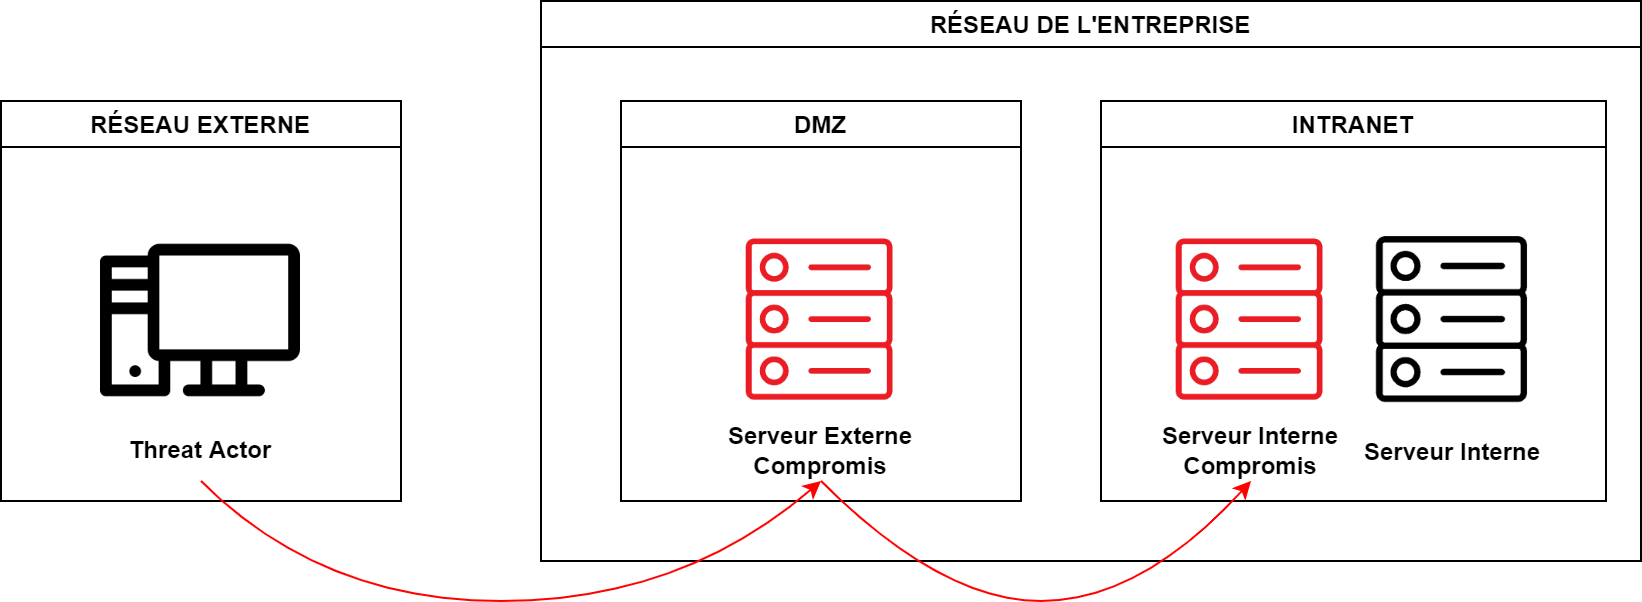
\includegraphics[width=0.95\linewidth]{images/attack-bridge/attack-bridge.png}
        }
    }
    \caption{Utilisation d'un serveur externe compromis comme pont pour entrer dans le réseau de l'entreprise.}
    \label{fig:attack-bridge}
\end{figure}

\begin{example}
    \hspace{0.45cm} Par exemple, dans le cas où un attaquant aurait compromis un serveur situé dans la DMZ (\textit{demilitarized zone}, zone démilitarisée en français) fournissant des services à la fois sur internet et sur le réseau interne de l'entreprise, il pourrait ensuite l'utiliser comme \textit{pont} pour rentrer dans le réseau interne de l'entreprise et y contaminer d'autres serveurs.

    Dans ce cas, les connexions réseaux de ce serveur compromis pourraient aider à déterminer quelles autres machines dans le réseau ont été compromises. Cette information se trouve presque toujours dans la RAM (et potentiellement dans le pare-feu ou dans les logs).
\end{example}

Sur la figure \ref{fig:device-physicalmemory}, on peut voir les objets NT gérés par l'Object Manager. Un driver avec des privilèges administrateurs peut accéder à la mémoire RAM directement via l'API WIN32 et ainsi la copier sur le disque. C'est ainsi que tous les outils de capture RAM fonctionnent.

% https://en.wikipedia.org/wiki/Object_Manager_(Windows)

\begin{figure}
    \centering
    \makebox[\textwidth]{
        \resizebox{18cm}{!}{
            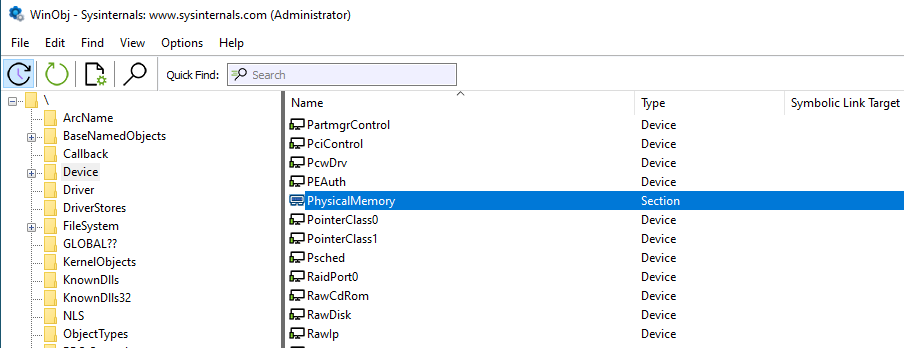
\includegraphics{images/RAM/WinObj-PhysicalMemory-Emplacement-RAM.png}
        }
    }
    \caption{Image de WinObj (de Sysinternals) montrant l'objet \textit{PhysicalMemory} auquel il faut accéder pour faire une image de la RAM.}
    \label{fig:device-physicalmemory}
\end{figure}



\subsection{Acquisition de la mémoire non-volatile}

Pour démarrer cette section, je vais tenter l'exercice de définir les données non-volatiles:

\begin{customquote}
    \hspace{0.45cm} Les données non-volatiles sont des données qui sont stockées sur la mémoire de masse. Elles ne sont donc pas perdues une fois que le système perd son alimentation électrique. Cependant, leur nature peut toujours être dynamique comme les logs qui peuvent être écrasés lorsque de nouveaux événements se produisent.
\end{customquote}

Contrairement à la mémoire RAM, la copie d'un disque peut également se faire lorsque le système est éteint. On peut même retirer le disque d'une machine éteinte pour le copier à l'aide d'un appareil forensique, ce qui évite totalement le risque d'écraser des données

Contrairement à la RAM, les données non-volatiles peuvent être extraites de la machine de plusieurs manières différentes. On peut, bien sûr, les copier avec un logiciel alors que le système est allumé. Par exemple, juste après avoir acquis une copie de la mémoire volatile. Mais elles peuvent aussi être copiées lorsque la machine est éteinte. On peut la redémarrer en bootant sur un autre système d'exploitation, situé sur une clé USB par exemple. Ou encore mieux, en retirant le disque dur de la machine pour le copier, de préférence en utilisant du matériel adapté à l'acquisition forensique. Toutes ces méthodes ne se valent pas d'un point de vue forensique, elles sont représentées sous la forme d'une pyramide sur la figure \ref{fig:non-volatile-memory} avec les méthodes préservant au mieux les données à la base et celles les préservant moins bien au sommet.

\begin{figure}
    \centering
    \makebox[\textwidth]{
        \resizebox{16cm}{!}{
            \includestandalone{images/pyramid-non-volatile-data/pyramid.tex}
        }
    }
    \caption{Pyramide des méthodes d'extraction des données non-volatiles.}
    \label{fig:non-volatile-memory}
\end{figure}

Parce que le stage a une durée limitée, j'ai décidé de me concentrer sur l'acquisition à chaud avec un disque externe, c'est-à-dire en branchant un disque dur externe lorsque le système est allumé et en utilisant un logiciel. L'avantage de cette méthode est qu'elle peut être utilisée juste après avoir effectué l'acquisition des données volatiles. Elle ne nécessite pas de connaître le mot de passe du BIOS ou de démonter l'ordinateur et elle est beaucoup plus rapide que lorsqu'on transfère les données via le réseau.



